\chapter{SISTEM BASIS DATA}

Karena sistem informasi ini akan menampilkan status pembayaran dari pajak bumi dan bangunan sektor perdesaan dan perkotaan, maka sistem basis data yang digunakan adalah sama dengan sistem basis data yang digunakan pada SISMIOP (Sistem Manajemen Informasi Objek Pajak), karena sistem ini sebetulnya telah mengakomodir pencatatan pembayaran yang berbasis aplikasi \textit{desktop}, aplikasi ini hanya melakukan akses terhadap data pencatatan pembayaran dengan berbasiskan \textit{web} sehingga memungkinkan dapat diakses oleh masyarakat wajib pajak.

Aplikasi SISMIOP menggunakan sistem basis data Oracle 11g, namun tidak seluruh tabel digunakan untuk menampilkan informasi mengenai status pembayaran pajak bumi dan bangunan sektor perdesaan dan perkotaan, hanya beberapa tabel saja yang digunakan seperti pada daftar berikut :

\begin{itemize}
	\item Tabel SPPT
	
Tabel SPPT ini nantinya digunakan untuk menampilkan tahun pajak serta besar tagihan pajak terhutang untuk pajak bumi dan bangunan sektor perdesaan dan perkotaan, dan menampilkan status pembayaran untuk tiap tahun pajaknya, apabila muncul tagihan yang belum terbayarkan setelah melewati masa jatuh tempo, maka atas dasar besarnya pokok ketetapan pada tabel ini pula akan dihitungkan jumlah sanksi administrasinya berupa denda setiap bulan sebesar 2\% (dua persen) untuk maksimal 15 (lima belas) bulan.	
	
	\item Tabel DAT\_OBJEK\_PAJAK
	
Tabel DAT\_OBJEK\_PAJAK ini diakses untuk menampilkan informasi objek pajak terbaru yang tercetak dalam lembar Surat Pemberitahuan Pajak Terhutang yang diterbitkan tiap tahun. 

Data ini ditampilkan sebagai bahan verifikasi data apabila pernah melakukan perubahan data, sehingga subjek pajak atau wajib pajak dapat melakukan konfirmasi ke bagian pelayanan pajak daerah.	
	
	\item Tabel DAT\_SUBJEK\_PAJAK
	
Tabel DAT\_SUBJEK\_PAJAK ini diakses untuk menampilkan informasi subjek pajak terbaru yang dapat ditetapkan sebagai wajib pajak pada lembar Surat Pemberitahuan Pajak Terhutang (SPPT) untuk jenis pajak bumi dan bangunan sektor perdesaan dan perkotaan.

Data ini pun ditampilkan sebagai bahan verifikasi data apabila pernah melakukan perubahan data yang biasanya akibat mutasi objek pajak, sehingga subjek pajak atau wajib pajak dapat melakukan konfirmasi ke bagian pelayanan pajak daerah.	
	
	\item Tabel REF\_KECAMATAN
	
Tabel REF\_KECAMATAN diakses untuk menampilkan nama Kecamatan dari objek pajak yang diakses oleh pengguna.	
	
	\item Tabel REF\_KELURAHAN
	
Tabel REF\_KELURAHAN diakses untuk menampilkan nama Kelurahan dari objek pajak yang diakses oleh pengguna.	
	
\end{itemize}

Diagram relasi tabel untuk tabel-tabel di atas adalah seperti pada gambar \ref{fig:db-diagram} berikut ini :

\begin{figure}[H]
	\centering
	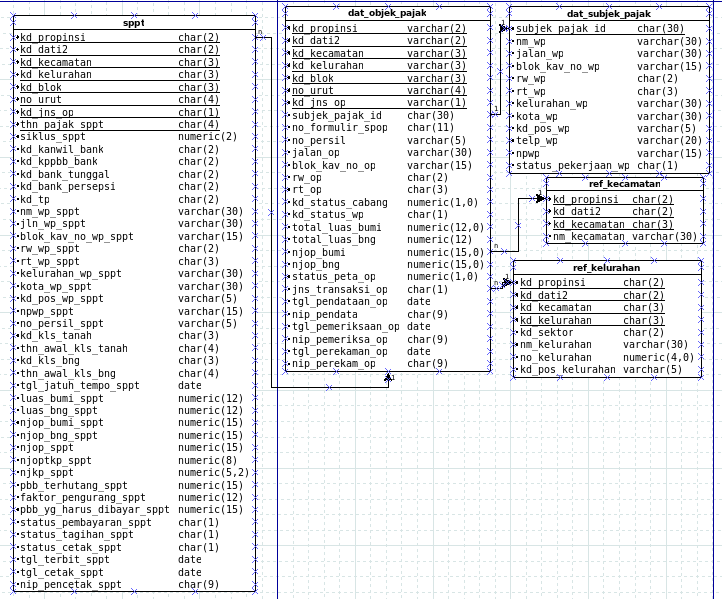
\includegraphics[width=1\textwidth]{./resources/db-diagram}
	\caption{Diagram Relasi Antar Tabel}
	\label{fig:db-diagram}
\end{figure}